\chapter{Fondamenti di GPGPU}\label{chap:fundamentals}

\section{Architettura di un programma GPGPU}
L'architettura di un programma GPGPU è composta da tre componenti principali: 
\begin{description}
    \item[Host] Il processore centrale (CPU) che esegue il codice principale del programma e gestisce la comunicazione con la GPU.
    \item[Device] La GPU, che esegue i kernel (flussi di esecuzione parallela) e gestisce la memoria dedicata.
    \item[Compute Unit (CU)] Un'unità di elaborazione all'interno della GPU che esegue i kernel in parallelo. Ogni CU contiene più core di elaborazione, che possono eseguire kernel in parallelo.
\end{description}

\begin{figure}[htbp]
    \centering
    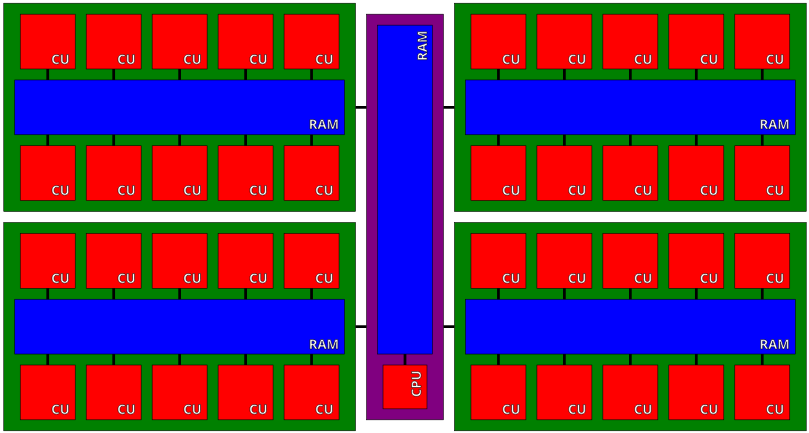
\includegraphics[width=0.8\textwidth]{images/gpgpu_architecture.png}
    \caption{Architettura di un sistema OpenCL, con CPU in viola(host) e diverse GPU (device) in verde che comunicano tra loro.}
    \label{fig:gpgpu_architecture}
\end{figure}

\subsection{Kernel, work-item e work-group}
Un kernel è una sequenza di istruzioni che può essere eseguita in parallelo su più compute unit della GPU. Ogni istanza di esecuzione del kernel è detta \textbf{work-item} (in CUDA vengono chiamati "thread") e ogni work-item che appartengono allo stesso \textbf{work-group} (un gruppo di work-item) condividono la memoria locale e possono sincronizzarsi tra loro. 

La collezione di tutti i work-item che eseguono un kernel è chiamata \textbf{launch grid} (o, in OpenCL, "NDRange"). La dimensione del launch grid è definita in termini di numero di work-item e work-group, e può essere configurata per massimizzare l'efficienza dell'esecuzione del kernel sulla GPU.

\section{Stream-Processing}
La prima forma di parallelismo su GPU è lo \emph{stream-processing}, in cui i dati vengono elaborati in flussi (streams) e ogni elemento del flusso viene elaborato in parallelo. Questo modello è adatto per operazioni che possono essere eseguite in modo indipendente su ciascun elemento, come ad esempio l'elaborazione di immagini o la simulazione di particelle, e rientra nella categoria del parallelismo \emph{data-based}.

\subsection{Kernel e dati}
In questo caso il kernel è la sequenza di istruzioni da eseguire su porzioni corrispondenti di più input stream per ottenere uno stream di output. Il kernel lavora solo con i dati che gli sono stati assegnati, e non ha accesso a dati al di fuori del suo work-item o work-group.

In particolare, le operazioni che possono essere eseguite in parallelo sono quelle per cui il risultato delle operazioni è indipendente dalla gestione della divisione e della elaborazione dei dati, processi entrambi gestiti interamente dall'hardware. Quest'ultima caratteristica fa sì che lo stream processing effettuato su determinati dati eseguendo delle date operazioni abbia lo stesso risultato indipendentemente dall’hardware utilizzato (cambia solamente il tempo impiegato).

Il programmatore non ha alcun controllo sulla divisione del lavoro tra i work-item o tra i work-group e non può sincronizzare i work-item tra loro, se non quelli appartenenti allo stesso work-group.

\subsection{Esempio: Mandelbrot fractal}
Il frattale di Mandelbrot è un insieme di punti complessi che non diverge quando iterati attraverso una funzione quadratica. Per generare un'immagine del frattale, ogni pixel dell'immagine può essere calcolato indipendentemente, rendendo questo problema ideale per il parallelismo su GPU.

\begin{figure}[htbp]
    \centering
    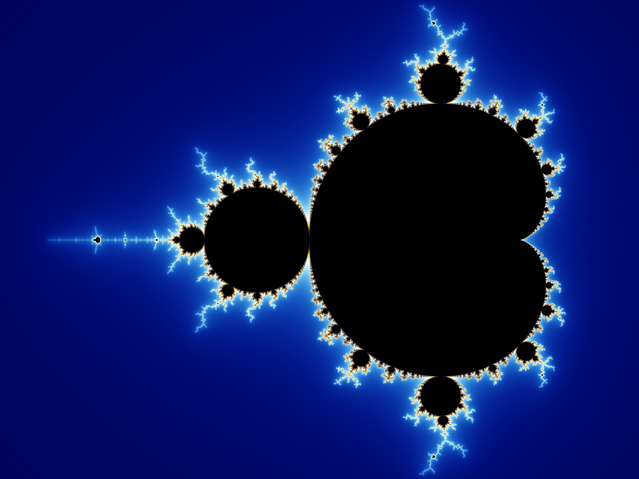
\includegraphics[width=0.8\textwidth]{images/mandelbrot_fractal.png}
    \caption{Frattale di Mandelbrot generato utilizzando il parallelismo su GPU.}
    \label{fig:mandelbrot}
\end{figure}

\noindent
Si può rapresentare la serie di questo frattale come
\[
z_{n+1} = z_n^2 + c
\]
dove \(z\) è un numero complesso e \(c\) è un punto complesso che rappresenta la posizione del pixel nell'immagine. Il kernel calcola il numero di iterazioni necessarie affinché \(z\) diverga (superi un certo limite) per ogni pixel, e questo numero di iterazioni viene utilizzato per determinare il colore del pixel nell'immagine finale.

\paragraph{Versione seriale.}
La versione seriale del codice per generare il frattale di Mandelbrot potrebbe essere scritta come:

\begin{code}[caption={Programma seriale per il calcolo dell'insieme di Mandelbrot},label={lst:mandelbrot}]
int nrows, ncols, maxiter;
float xmin, xmax, ymin, ymax;
int *bitmap;

for (int row = 0; row < nrows; ++row) {
    for (int col = 0; col < ncols; ++col) {
        complex z, c;
        int iter;

        c.real = xmin + col*(xmax - xmin)/ncols;
        c.img  = ymin + row*(ymax - ymin)/nrows;

        z = c;

        for (iter = 0; iter < maxiter; ++iter) {
            z = add(mul(z, z), c); /* z_{n+1} = z_n^2 + c */
            if (norm(z) > 2)
                break;
        }

        bitmap[row*ncols + col] = !!(iter < maxiter);
    }
}
\end{code}

Il core parallelizzabile di questo codice è il doppio ciclo annidato che itera su ogni pixel dell'immagine. Ogni iterazione del ciclo interno calcola il numero di iterazioni necessarie affinché \(z\) diverga per un pixel specifico, e questo calcolo può essere eseguito in parallelo per tutti i pixel dell'immagine. Questo può essere considerato un candidato ideale per scrivere un kernel che esegue il calcolo in parallelo su una GPU, dove ogni work-item si occupa di calcolare il numero di iterazioni per un pixel specifico.

\section{Memoria}
I device di calcolo hanno la propria memoria dedicata, che è separata dalla memoria del host. Gli spazi di memoria presenti sulla GPU sono diversi:
\begin{description}
    \item[Global Memory] La memoria globale è accessibile a tutti i work-item e work-group, ma ha una latenza elevata. I contenuti in essi presenti permangono per la durata di esecuzione dell'intero programma e i dati possono essere modificati dai kernel.
    \item[Constant Memory] La memoria costante è una porzione di memoria globale che è ottimizzata per il broadcasting. Può essere modificata solo dall'host e se necessario può essere cambiata tra l'esecuzione di un kernel e l'altro.
    \item[Images (o texture in CUDA)] La memoria per le immagini è ottimizzata per l'accesso 2D e 3D, e supporta operazioni di filtraggio, interpolazione,  l'indexing multidimensionale e la normalizzazione delle coordinate.
    \item[Local Memory (shared memory in CUDA)] La memoria locale si trova fisicamente sulle compute unit e, a differenza della memoria globale, è volatile e viene allocata all'inizio di un determinato kernel e successivamente svuotata. Può essere comunque utilizzata dai work-item appartenenti allo stesso work-group per condividere dati e sincronizzarsi tra loro. Viene utilizzata per algoritmi più complessi che richiedono la condivisione di dati tra i work-item, come ad esempio le operazioni di riduzione o di convoluzione, e permette di eseguire su CPU algoritmi non imbarazzantemente paralleli.
    \item[Private memory (local memory in CUDA)] Questa memoria contiene dati temporanei specifici di un singolo work-item, tipitcamente i dati da inserire all'interno dei registri di esecuzione. Se non vi sono registri sufficienti per la quantità di dati da gestire si ha un \emph{register spill}\footnote{Il register spill è un fenomeno che si verifica quando un kernel utilizza più registri di quelli disponibili sulla GPU, costringendo il compilatore a spostare alcuni dati dalla memoria dei registri alla memoria globale o locale. Questo può causare un degrado delle prestazioni, poiché l'accesso alla memoria globale o locale è molto più lento rispetto all'accesso ai registri.} e i dati vengono spostati in local memory, con conseguente degrado delle prestazioni.
\end{description}

\section{Struttura di un programma GPGPU}

\subsection{Pipeline di esecuzione}
Un programma GPGPU è composto da 4 parti principali:
\begin{description}
    \item[Selects.] - Selezione del dispositivo di calcolo (GPU) su cui eseguire il programma. In questo caso CUDA fa tutto a runtime dietro le quinte, mentre OpenCL richiede al programmatore di specificare esplicitamente il dispositivo da utilizzare. 
    Esempio: se si dispone di più GPU, è possibile selezionare quella più adatta per l'esecuzione del programma, ad esempio in base alla quantità di memoria disponibile o alla potenza di calcolo.
    \item[Uploads.] - Trasferimento dei dati dal host alla GPU. Questo passaggio è necessario perché la GPU ha la propria memoria dedicata e non può accedere direttamente alla memoria del host.
    Esempio: se si sta elaborando un'immagine, è necessario caricare i dati dell'immagine nella memoria della GPU prima di eseguire il kernel che elabora l'immagine.
    \item[Runs.] - Esecuzione del kernel sulla GPU. In questo passaggio, il kernel viene lanciato sulla GPU e i work-item eseguono il codice in parallelo. 
    Esempio: se si sta calcolando il frattale di Mandelbrot, è necessario lanciare un kernel che esegue il calcolo per ogni pixel dell'immagine in parallelo.
    \item[Downloads.] - Trasferimento dei dati dalla GPU al host. Dopo l'esecuzione del kernel, i risultati devono essere trasferiti nuovamente al host per essere utilizzati o visualizzati.
    Esempio: se si sta elaborando un'immagine, è necessario scaricare i dati dell'immagine elaborata dalla memoria della GPU al host per visualizzarla o salvarla su disco. 
\end{description}\

\subsection{Comunicazione host-device}
Considerando un setup moderno:
\begin{itemize}
    \item Bandwidth host: 50 GB/s (PCIe 4.0 x16)
    \item Bandwidth device: 900 GB/s (HBM2)
\end{itemize}

\noindent
Il problema principale di questo tipo di architettura è che la comunicazione tra host e device è molto più lenta rispetto alla comunicazione all'interno del device stesso. Pertanto, è importante minimizzare il numero di trasferimenti di dati tra host e device per massimizzare le prestazioni del programma GPGPU.
In particolare, il trasferimento dati da host a GPU dipende dalla banda passante del bus PCI express, che si aggira sui 16 GB/s.

\begin{figure}[htbp]
    \centering
    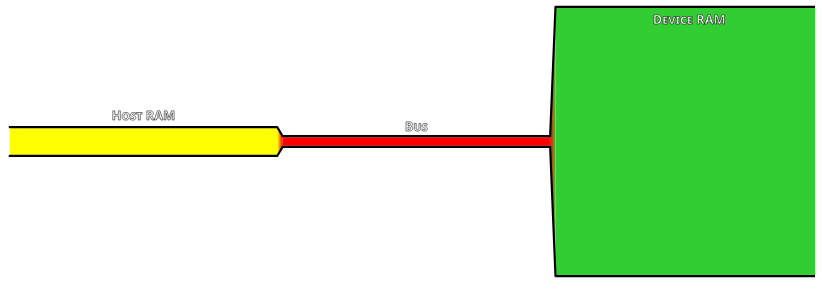
\includegraphics[width=0.8\textwidth]{images/host_device_communication.png}
    \caption{Comunicazione tra host e device, con i trasferimenti di dati che avvengono attraverso il bus PCIe.}
    \label{fig:host_device_communication}
\end{figure}

\subsection{Sorgente singolo e separato}
Come già accennato, un programma GPGPU è composto da due parti distinte: il codice \emph{host}, eseguito sulla CPU, e il codice \emph{device}, costituito dai kernel che verranno eseguiti sulla GPU. Queste due componenti non solo vengono eseguite su architetture differenti, ma sono anche tradotte in linguaggi macchina distinti; inoltre, tale linguaggio può variare anche tra diverse generazioni di GPU dello stesso produttore.

\begin{figure}[htbp]
    \centering
    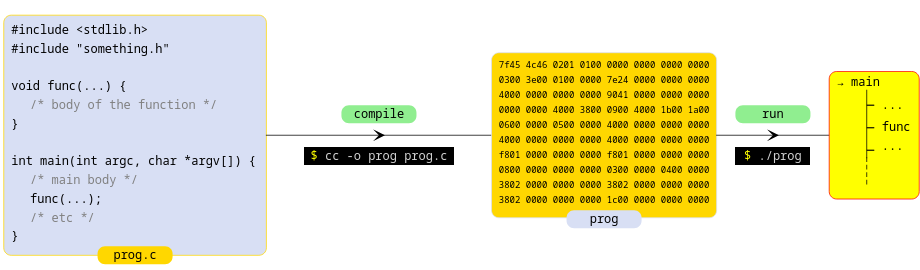
\includegraphics[width=0.8\textwidth]{images/classic_source_structure.png}
    \caption{Processo di compilazione ed esecuzione di un programma C: dal codice sorgente alla generazione dell'eseguibile e alla sua esecuzione.}
    \label{fig:single_separate_source}
\end{figure}

Il modo in cui queste due parti vengono organizzate e compilate porta a distinguere due approcci principali: il modello \emph{single-source} e il modello \emph{separate-source}.

\paragraph{Single-source.}
Nel modello \emph{single-source}, tipico ad esempio di CUDA, il codice host e quello device convivono all'interno dello stesso file sorgente. In questo caso è il compilatore a occuparsi automaticamente di separare le due componenti e di gestirne la compilazione.

Più precisamente, le funzioni destinate all'esecuzione sulla GPU vengono identificate tramite annotazioni specifiche, come \texttt{\_\_global\_\_}. Il compilatore (ad esempio \texttt{nvcc}) analizza il sorgente e lo suddivide in una parte host, che viene passata al compilatore tradizionale, e una parte device, che viene compilata con un backend dedicato alla GPU. Il risultato è la produzione di due codici macchina distinti, uno per la CPU e uno per il device.

\begin{figure}[htbp]
    \centering
    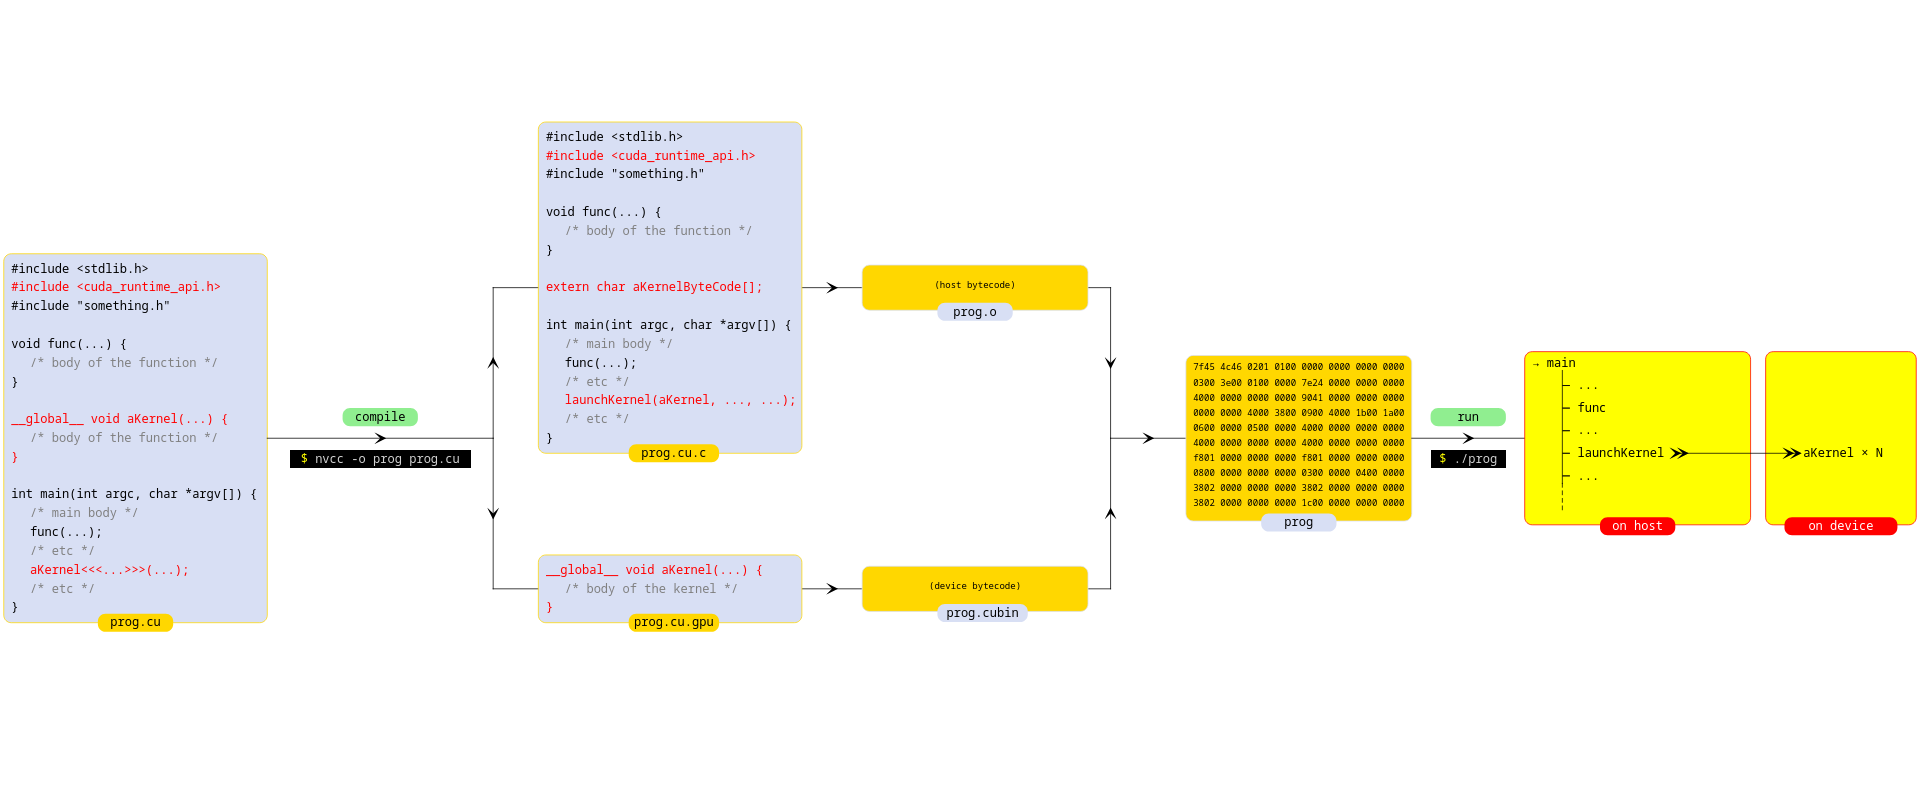
\includegraphics[width=1\textwidth]{images/single_source_structure.png}
    \caption{Processo di compilazione ed esecuzione in CUDA: il codice single-source viene separato in componente host e device, compilato in bytecode distinti e ricombinato in un unico eseguibile che coordina CPU e GPU.}
    \label{fig:single_source_structure}
\end{figure}

Dal punto di vista dell'esecuzione, il codice host può invocare un kernel tramite una sintassi dedicata, come \texttt{aKernel<<<...>>>();}, specificando la configurazione della griglia di esecuzione. È importante osservare che il lancio del kernel è asincrono rispetto all'host: questo significa che l'host continua la propria esecuzione senza attendere il completamento del kernel, e quindi una misura del tempo attorno al lancio non rappresenta il tempo reale di esecuzione sul device.

Questo approccio risulta generalmente più semplice da utilizzare, in quanto riduce la quantità di codice da gestire e garantisce coerenza tra i tipi di dato utilizzati lato host e lato device. Tuttavia, introduce alcuni vincoli: richiede l'uso di un compilatore specifico, che deve essere compatibile con il compilatore host, e impone di specificare a priori il device di destinazione. Inoltre, non consente una compilazione selettiva dei singoli kernel.

\paragraph{Separate-source.}
Nel modello \emph{separate-source}, adottato ad esempio in OpenCL, il codice device è completamente separato da quello host e viene gestito come entità indipendente.

In questo caso, i kernel risiedono tipicamente in file distinti oppure vengono rappresentati come stringhe all'interno del codice host. Durante l'esecuzione, è il programma host a caricare il sorgente dei kernel e a richiederne la compilazione al driver della GPU. La compilazione avviene quindi a runtime, e non in fase di build, rendendo questo approccio più dinamico e flessibile. I driver, per ottimizzare le prestazioni, mantengono generalmente una cache dei kernel già compilati, evitando di ripetere operazioni costose.

\begin{figure}[htbp]
    \centering
    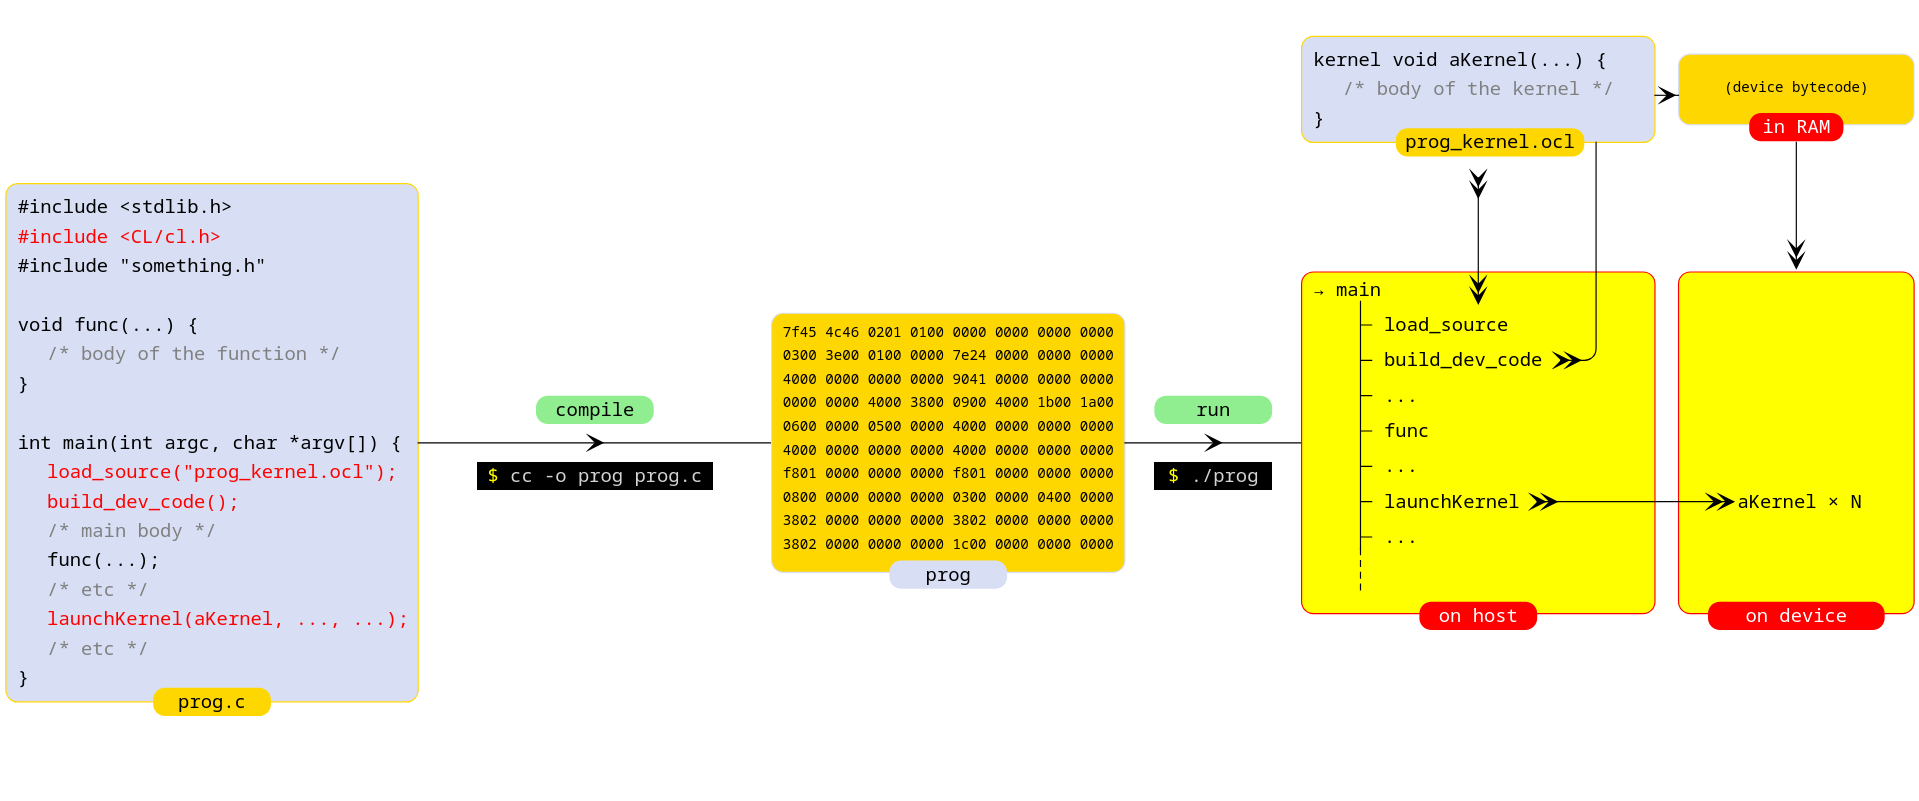
\includegraphics[width=1\textwidth]{images/separate_source_structure.png}
    \caption{Processo di compilazione ed esecuzione in OpenCL: il codice host viene compilato separatamente, mentre i kernel device sono caricati e compilati a runtime dal driver prima dell'esecuzione sulla GPU.}
    \label{fig:separate_source_structure}
\end{figure}

Questo modello offre una maggiore portabilità, in quanto lo stesso codice device può essere compilato su architetture differenti e non richiede l'uso di un compilatore specifico per l'host. Inoltre, permette di selezionare dinamicamente quali kernel compilare ed eseguire.

D'altra parte, questa flessibilità comporta un aumento della complessità: il codice da gestire è maggiore e la separazione tra host e device rende meno immediata la condivisione dei tipi di dato, che devono quindi essere definiti con particolare attenzione, privilegiando strutture semplici e compatibili tra i due ambienti.

\section{Stream Computing}
Lo stream computing è un paradigma di programmazione che si basa sull'elaborazione di flussi di dati in tempo reale. In questo modello, i dati vengono elaborati in modo continuo e parallelo, consentendo di ottenere prestazioni elevate e bassa latenza.

\subsection{Hardware e controller}
Le GPU sono \textbf{progettate} per lo stream computing. Una singola compute unit può gestire centinaia di work-item che eseugono lo stesso kernel su più dati in parallelo. La memoria globale, inoltre, ha un'ampia banda passante ma anche alta latenza, per questo motivo si devono usare dei pattern di accesso ottimali per massimizzare le prestazioni. Le GPU sono anche asincrone rispetto alla CPU, il che significa che è possibile eseguire più kernel in parallelo e sovrapporre l'esecuzione dei kernel con i trasferimenti di dati tra host e device.

Il controller di una GPU è responsabile della gestione dell'esecuzione dei kernel e della comunicazione tra host e device. Il controller gestisce la coda dei kernel da eseguire, assegna i work-item alle compute unit e gestisce i trasferimenti di dati tra host e device. Generalmente è un dispositivo ad \textbf{alta latenza} e questo influenza le strutture dati utilizzabile che devono essere efficienti da accedere, ha però un'\textbf{alta banda passante} che consente di trasferire grandi quantità di dati in parallelo.

\subsection{SPMD, SIMD e SIMT}

Nel contesto del calcolo parallelo su GPU, è importante distinguere tra diversi modelli di esecuzione che descrivono come le operazioni vengono applicate ai dati. I paradigmi più rilevanti sono \emph{SIMD}, \emph{SPMD} e \emph{SIMT}, che, pur essendo correlati, rappresentano livelli di astrazione differenti.
\begin{description}
\item[SIMD] Il paradigma \emph{Single Instruction Multiple Data} (SIMD) è tipico delle CPU moderne. In questo modello, una singola istruzione viene applicata simultaneamente a più dati organizzati in vettori. Il programmatore deve esplicitamente utilizzare tipi vettoriali (ad esempio \texttt{float4}, \texttt{float8}, ecc.) e scrivere codice che sfrutti direttamente la larghezza delle unità SIMD.

Questo approccio richiede una certa conoscenza dell'hardware sottostante: per sfruttare pienamente le prestazioni, è necessario adattare il codice alla larghezza dei registri vettoriali (ad esempio SSE, AVX, AVX2). Di conseguenza, il codice risulta meno portabile e più difficile da mantenere.

\item[SPMD] Il paradigma \emph{Single Program Multiple Data} (SPMD) rappresenta un modello di programmazione più astratto. In questo caso, il programmatore scrive un singolo programma (il kernel), che viene eseguito molte volte in parallelo su dati diversi. Ogni istanza di esecuzione (work-item) esegue lo stesso codice, ma opera su porzioni differenti dei dati.

Questo modello è particolarmente adatto alla programmazione su GPU, in quanto consente di esprimere facilmente il parallelismo senza preoccuparsi direttamente della gestione delle unità vettoriali.

\item[SIMT] Dal punto di vista hardware, le GPU implementano un modello chiamato \emph{Single Instruction Multiple Threads} (SIMT), che può essere visto come una realizzazione efficiente del modello SPMD. Il programmatore scrive codice come se ogni work-item fosse indipendente, ma l'hardware esegue gruppi di work-item (chiamati \emph{warp} in NVIDIA o \emph{wavefront} in AMD) in maniera sincronizzata, condividendo lo stesso flusso di istruzioni.

Questo significa che, anche se il codice sembra scalare (operare su singoli dati), viene in realtà eseguito in modo simile al SIMD, ma con una gestione trasparente da parte dell'hardware. Tuttavia, il controllo di flusso è limitato: se i thread all'interno dello stesso gruppo seguono percorsi diversi (branch divergenti), le istruzioni vengono serializzate, con una perdita di prestazioni.
\end{description}

\paragraph{Esempio}
La differenza tra SIMD e SPMD/SIMT può essere illustrata con un semplice esempio di somma tra vettori.

Nel caso SIMD (tipico su CPU), il programmatore lavora esplicitamente su vettori:
\begin{code}
float4 a, b, c;
a = /* load vector */;
b = /* load vector */;
c = a + b;
\end{code}

Nel caso SPMD/SIMT (tipico su GPU), il programmatore scrive invece codice scalare, che verrà eseguito in parallelo su molti elementi:
\begin{code}
float a, b, c;
a = /* load scalar */;
b = /* load scalar */;
c = a + b;
\end{code}

In questo secondo caso, è l'hardware della GPU a replicare automaticamente l'esecuzione su molti dati e a distribuirla tra le unità di calcolo disponibili.

\subsection{Wide cores}
Le GPU sono progettate con un gran numero di core, ma ciascun core è relativamente semplice rispetto a quelli di una CPU. Questo approccio architetturale privilegia il throughput complessivo rispetto alla complessità del singolo core, rendendo le GPU particolarmente efficienti per carichi di lavoro altamente paralleli. Più precisamente, un multiprocessore della GPU (Compute Unit o Streaming Multiprocessor) contiene numerosi \emph{processing elements} (PE), che possono essere visti come unità di calcolo elementari. Tuttavia, questi elementi non operano in modo completamente indipendente: essi eseguono lo stesso flusso di istruzioni in maniera coordinata, secondo un modello simile al SIMD, ma con una gestione demandata all'hardware.

Questa organizzazione introduce alcune limitazioni sul controllo di flusso. In particolare, le GPU sono ottimizzate per schemi di esecuzione regolari, dove tutti i work-item seguono lo stesso percorso. Costrutti complessi come branching irregolare o ricorsione sono poco efficienti o addirittura non supportati. Per gestire le divergenze, l'hardware utilizza tecniche come la \emph{predication} e il \emph{lane masking}, che permettono di eseguire comunque le istruzioni, ma disabilitando selettivamente alcuni work-item, con un possibile degrado delle prestazioni.

Un aspetto fondamentale è che i work-item non vengono eseguiti singolarmente, ma in gruppi a dimensione fissa. Questi gruppi sono chiamati \emph{warp} nell'architettura NVIDIA e \emph{wavefront} in quella AMD, e rappresentano la larghezza effettiva del parallelismo hardware (SIMT width). I work-item all'interno dello stesso gruppo vengono eseguiti in \emph{lock-step}, ovvero condividono lo stesso contatore di programma e avanzano insieme nell'esecuzione.

\subsection{Strutture dati ideali}
L'efficienza di un programma GPGPU dipende in maniera significativa da come i dati sono organizzati in memoria. A differenza delle CPU, dove il costo dell'accesso alla memoria è in parte nascosto da cache sofisticate, nelle GPU è fondamentale strutturare i dati in modo da sfruttare al meglio la banda disponibile.

\paragraph{Tipologie di dati.}
Un primo aspetto riguarda la scelta dei tipi di dato. Le GPU sono ottimizzate per operare su dati di dimensione ben definita, tipicamente 32, 64 o 128 bit. Per questo motivo, è spesso conveniente utilizzare tipi vettoriali (come \texttt{float2}, \texttt{float4}, ecc.), che permettono di allineare meglio i dati e sfruttare in modo più efficiente le operazioni di lettura e scrittura.

\paragraph{Layout in memoria.}
Un secondo aspetto fondamentale è il layout in memoria. I dati dovrebbero essere disposti in modo contiguo e correttamente allineato: in particolare, l'indirizzo di un dato dovrebbe essere un multiplo della sua dimensione. Ad esempio, un valore \texttt{float} (4 byte) viene letto in modo efficiente se il suo indirizzo è multiplo di 4. Un accesso non allineato può richiedere più transazioni di memoria, con un conseguente peggioramento delle prestazioni.

\paragraph{Accessi coalescenti.}
Infine, è importante considerare che gli accessi alla memoria non avvengono a livello di singolo work-item, ma a livello di gruppi di esecuzione (warp o wavefront). I work-item all'interno dello stesso gruppo eseguono la stessa istruzione in parallelo e, idealmente, accedono a posizioni contigue di memoria. In questo caso, il controller di memoria può soddisfare tutte le richieste con una singola transazione, massimizzando la banda passante. Al contrario, accessi irregolari o non contigui portano a un aumento del numero di transazioni e quindi a una riduzione delle prestazioni.

\subsubsection*{Esempi di accesso alla memoria}
Un errore comune consiste nell’utilizzare strutture dati che sono naturali dal punto di vista logico, ma inefficienti dal punto di vista dell’accesso alla memoria. Consideriamo ad esempio una simulazione di particelle:

\begin{code}
typedef struct particle {
    float3 pos;
    float3 vel;
} particle_t;

kernel void iteration(global particle_t *particles)
{
    int workitem = get_global_id(0);
    float3 pos = particles[workitem].pos;
    float3 vel = particles[workitem].vel;
    /* do stuff */
}
\end{code}

In questo caso, ogni work-item accede ai campi \texttt{pos} e \texttt{vel} della propria particella. Tuttavia, i dati in memoria sono interleavati (Array of Structures), e quindi i work-item di uno stesso warp non accedono a locazioni contigue per ciascun campo. Questo porta a accessi non coalescenti e a un aumento del numero di transazioni di memoria.

\paragraph{Caso inefficiente (Array of Structures)}
\begin{figure}[htbp]
    \centering
    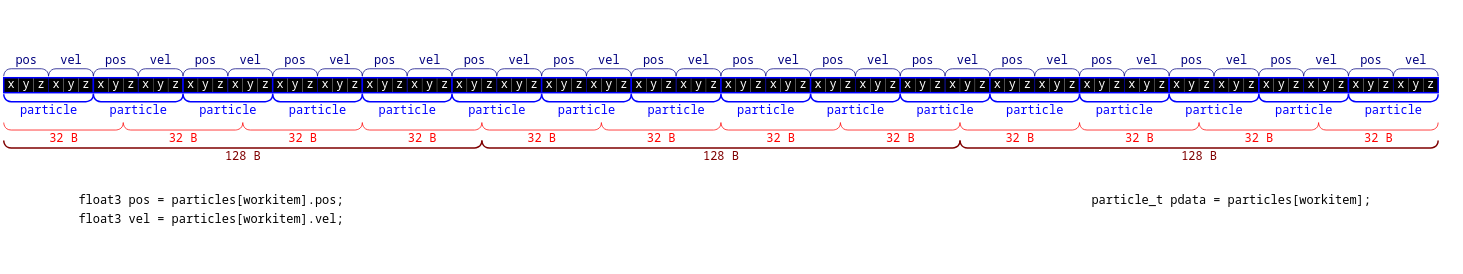
\includegraphics[width=\textwidth]{images/aos_bad.png}
    \caption{Accesso inefficiente con layout Array of Structures: i campi \texttt{pos} e \texttt{vel} sono interleavati, causando accessi non coalescenti e multiple transazioni di memoria per warp.}
    \label{fig:aos_bad}
\end{figure}

Nel caso mostrato, i work-item accedono a campi distribuiti in memoria in modo non contiguo. Il controller di memoria non può aggregare le richieste e deve effettuare più transazioni, con conseguente perdita di prestazioni.

\paragraph{Caso intermedio (allineamento con float4)}
Un miglioramento consiste nell’utilizzare tipi allineati, ad esempio:

\begin{code}
typedef struct particle {
    float4 pos;
    float4 vel;
} particle_t;
\end{code}

\begin{figure}[htbp]
    \centering
    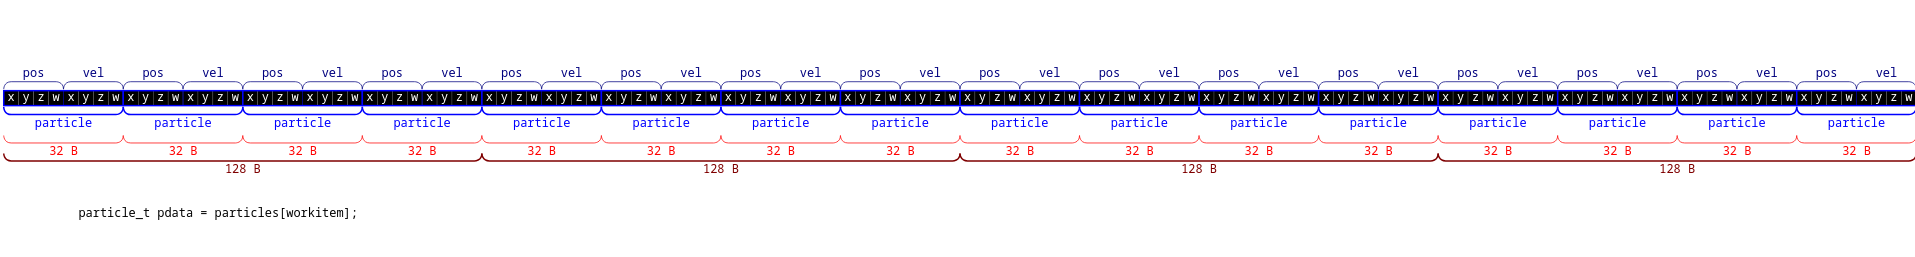
\includegraphics[width=\textwidth]{images/aos_aligned.png}
    \caption{Allineamento tramite \texttt{float4}: i dati sono meglio allineati e possono essere caricati con meno transazioni, ma il layout rimane di tipo AoS e non è ottimale.}
    \label{fig:aos_aligned}
\end{figure}

In questo modo, gli accessi sono più regolari e meglio allineati. Tuttavia, i dati restano organizzati come array di strutture, quindi non si ottiene ancora il massimo livello di efficienza.

\paragraph{Caso efficiente (Structure of Arrays)}
L’approccio più efficiente consiste nel separare i dati in più array (Structure of Arrays):

\begin{code}
kernel void iteration(
    global float4 * restrict posArray,
    global float4 * restrict velArray)
{
    int workitem = get_global_id(0);
    float4 pos = posArray[workitem];
    float4 vel = velArray[workitem];
    /* do stuff */
}
\end{code}

\begin{figure}[htbp]
    \centering
    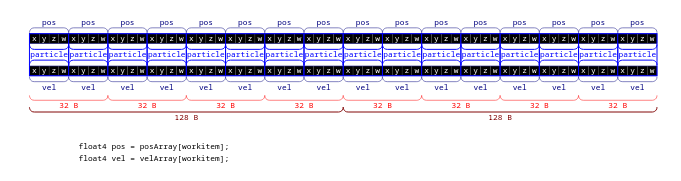
\includegraphics[width=\textwidth]{images/soa_good.png}
    \caption{Layout Structure of Arrays: i work-item accedono a dati contigui, permettendo accessi coalescenti e riducendo il numero di transazioni di memoria.}
    \label{fig:soa_good}
\end{figure}


In questo caso, i work-item di uno stesso warp accedono a elementi contigui degli array \texttt{posArray} e \texttt{velArray}. Il controller di memoria può quindi servire tutte le richieste con un numero minimo di transazioni (tipicamente una per array), massimizzando la banda passante.

\section{Asincronicità}

La GPU opera in maniera indipendente rispetto alla CPU, rendendo la comunicazione tra host e device intrinsecamente asincrona. Per gestire questa interazione, si utilizzano delle code di esecuzione chiamate \emph{command queues} in OpenCL e \emph{streams} in CUDA.

Mentre in CUDA la gestione può essere implicita, in OpenCL la gestione della coda deve sempre essere esplicitata. Per coordinare le operazioni vengono utilizzati gli \emph{eventi}, marcatori associati ai singoli comandi che permettono all'host di monitorare l'avanzamento dei singoli task. Nello specifico, l'host può:

\begin{itemize}
    \item Sospendere l'esecuzione di un comando fino al completamento di un altro task precedentemente avviato;
    \item Richiedere lo stato di un evento;
    \item Imporre delle barriere di sincronizzazione affinché un device completi tutti i comandi pendenti prima di procedere.
\end{itemize}

Il principale vantaggio dell’asincronicità risiede nella capacità di "nascondere" la latenza dei trasferimenti dati attraverso il bus PCIe sovrapponendo temporalmente le operazioni di I/O con l'esecuzione dei kernel.
Inoltre, gli eventi permettono una sincronizzazione granulare (sul singolo kernel) rispetto alla sincronizzazione globale dell'intero device.

\section{CUDA vs OpenCL}

CUDA e OpenCL rappresentano due approcci differenti alla programmazione su GPU. Pur condividendo molti concetti di base (kernel, memoria device, esecuzione parallela), si differenziano sia per il modello di programmazione lato host sia per il linguaggio utilizzato lato device.

\begin{table}[htbp]
\centering
\small
\begin{tabular}{lll}
\toprule
\textbf{Categoria} & \textbf{CUDA} & \textbf{OpenCL} \\
\midrule

\multicolumn{3}{l}{\textbf{Host API}} \\
\midrule
Supporto hardware & Solo GPU NVIDIA & Multi-vendor (CPU, GPU, FPGA) \\
Modello sorgente & Single-source & Separate-source \\
Compilazione kernel & Compile-time & Runtime (driver) \\
Gestione device & Implicita & Esplicita (platform, device, context) \\
Gestione code & Implicita & Esplicita (command queue) \\
Memoria device & Puntatori diretti & Buffer/oggetti astratti \\
Lancio kernel & Grid/block & NDRange (work-item/work-group) \\

\midrule
\multicolumn{3}{l}{\textbf{Device Language}} \\
\midrule
Linguaggio & C++ esteso & OpenCL C \\
Libreria standard & Limitata & Completa (built-in) \\
Swizzling vettori & Non supportato & Supportato (\texttt{f.xy}, ecc.) \\
Tipi vettoriali & Supportati & Supportati \\
Accesso agli indici & Manuale (\texttt{threadIdx}) & Built-in (\texttt{get\_global\_id}) \\

\bottomrule
\end{tabular}
\caption{Confronto tra CUDA e OpenCL.}
\label{tab:cuda_opencl}
\end{table}

\subsection{Differenze lato host}

Dal punto di vista dell’API host, CUDA è una piattaforma proprietaria sviluppata da NVIDIA e progettata per sfruttare al massimo le caratteristiche delle GPU di questo produttore. Questo si traduce in un modello più semplice e diretto: molte operazioni, come la gestione dei device e delle code di esecuzione, sono gestite implicitamente dal runtime. Inoltre, quando si alloca memoria sul device, viene restituito direttamente un puntatore utilizzabile nel codice CUDA.

OpenCL, al contrario, è uno standard aperto pensato per sistemi eterogenei. Questo comporta una maggiore flessibilità, ma anche una maggiore complessità. Il programmatore deve esplicitamente gestire piattaforme, device e code di esecuzione. Inoltre, la memoria allocata sul device non è accessibile tramite puntatori diretti, ma tramite oggetti astratti (buffer), che vengono gestiti attraverso l’API.

Un’altra differenza riguarda l’organizzazione del codice: CUDA adotta un modello \emph{single-source}, mentre OpenCL utilizza un approccio \emph{separate-source}, in cui i kernel vengono compilati a runtime.

\subsection{Differenze lato device}

Per quanto riguarda il linguaggio device, CUDA utilizza un’estensione del C++, mentre OpenCL definisce un proprio linguaggio basato sul C.

Nel caso di CUDA, il linguaggio è fortemente integrato con il modello di esecuzione, ma presenta alcune limitazioni: ad esempio, non esiste una vera libreria standard completa e non sono supportate alcune operazioni tipiche dei linguaggi vettoriali, come lo \emph{swizzling}. Inoltre, l’indice globale di un thread deve essere calcolato manualmente (combinando gli indici di blocco e thread) e la divisione della griglia di lancio in work group deve essere anch'essa effettuata manualmente.

OpenCL, invece, fornisce un linguaggio più ricco dal punto di vista delle operazioni vettoriali, offrendo costrutti come lo swizzling (ad esempio \texttt{f.xy}, \texttt{f.wwxx}), ed è dotato di funzioni built-in per ottenere automaticamente gli indici dei work-item e dei work-group. Inoltre, OpenCL possiede un meccanismo di estensioni che permettono di sfruttare le caratteristiche architetturali proprie di specifici hardware.